\documentclass{beamer}
%\usetheme{Madrid} % My favorite!
%\usetheme{Boadilla} % Pretty neat, soft color.	
\usetheme{default}
%\usetheme{Warsaw}
%\usetheme{Bergen} % This template has navigation on the left
%\usetheme{Frankfurt} % Similar to the default 
%with an extra region at the top.
%\usecolortheme{seahorse} % Simple and clean template
%\usetheme{Darmstadt} % not so good
% Uncomment the following line if you want %
% page numbers and using Warsaw theme%
% \setbeamertemplate{footline}[page number]
%\setbeamercovered{transparent}
%\setbeamercovered{invisible}
% To remove the navigation symbols from 
% the bottom of slides%
\setbeamertemplate{navigation symbols}{} 
%	
\usepackage{subfig}
\usepackage{amsmath, amsthm, amssymb}
\usepackage{float}
\usepackage{rotating}
\usepackage{graphicx}  
\usepackage{longtable} 
\usepackage{xcolor}
\usepackage{bm}
\usepackage{tikz}
\usetikzlibrary{shapes}
\tikzset{My Arrow Style/.style={single arrow, fill=red!50, anchor=base, align=center,text width=.5cm,rotate =270}}
\newcommand{\MyArrow}[2][]{\tikz[baseline] \node [My Arrow Style,#1] {#2};}
\tikzset{My 2Arrow Style/.style={single arrow, fill=red!50, anchor=base, align=center,text width=.5cm,rotate =90}}
\newcommand{\MyArrowUp}[2][]{\tikz[baseline] \node [My 2Arrow Style,#1] {#2};}
\newcommand{\bmat}{\begin{matrix}}
\newcommand{\emat}{\end{matrix}}

\newtheorem{acknowledgement}[theorem]{Acknowledgement}
\newtheorem{algorithm}[theorem]{Algorithm}
\newtheorem{assumption}{Assumption}
\newtheorem{axiom}{Axiom}
\newtheorem{case}[theorem]{Case}
\newtheorem{claim}[theorem]{Claim}
\newtheorem{conclusion}[theorem]{Conclusion}
\newtheorem{condition}[theorem]{Condition}
\newtheorem{conjecture}{Conjecture}
\newtheorem{criterion}[theorem]{Criterion}
\newtheorem{proposition}{Proposition}
\newtheorem{summary}[theorem]{Summary}
\newtheorem{exercise}{Exercise}
\newtheorem{notation}{Notation}
\newtheorem{remark}{Remark}
%\graphicspath{{graphs//}}

\title {Taxation, Debt and Redistribution}
\author{Anmol Bhandari, David Evans, Mikhail Golosov, Thomas J. Sargent}

\date{\today}
% \today will show current date. 
% Alternatively, you can specify a date.
%
\begin{document}
%
\begin{frame}
\titlepage

\end{frame}

\begin{frame}
\frametitle{What do we do ?}
We study optimal taxation under commitment with
\begin{itemize}
 \item \textbf{Heterogeneous agents}
 
 \quad \color{red}$\rightarrow$ \color{black}Agents  have different productivities
 
 \item \textbf{Incomplete markets}
 
 \quad \color{red}$\rightarrow$ \color{black}All agents trade a risk-free bond
 
 \item \textbf{Affine taxes}
 
 \quad \color{red}$\rightarrow$ \color{black}Government can levy a proportional tax on labor earnings + lumpsump (tax or transfer) 
 
 \item \textbf{Aggregate shocks}
 
 \quad \color{red}$\rightarrow$ \color{black}Shocks to productivities, government expenditure etc.

 \end{itemize}
\end{frame}


\begin{frame}
\frametitle{What are we after ?}

\begin{enumerate}
 \item How costly are debt levels ?
 \item What are the long run properties of optimal allocations ?
\item How should policy respond to aggregate shocks with heterogeneous cross sectional implications ?
\end{enumerate}
 Representative agent with linear taxes
\begin{itemize}
 \item Higher levels of debt are distortionary
 \item With incomplete markets the government accumulates assets overtime
 \end{itemize}
 
 \end{frame}
 
 \begin{frame}
 \frametitle{Redistribution and optimal transfers}
 \begin{itemize}
  \item Representative agent models impose restrictions on transfers
  \begin{itemize}
 \item Implicit motives for redistribution :  Poor people cant pay lumpsump taxes
  \item These constraints either \emph{almost} always bind (For eg: Lucas Stokey, AMSS) and are key for long run dynamics
  \end{itemize}
\item We begin with explicit redistribution motives but leave transfers to be determined optimally
 \end{itemize}

 \vspace{4mm}
 \color{red}\emph{The prescription for optimal tax-transfers are substantially different with explicit redistribution considerations}
 \end{frame}
 



\begin{frame}
\frametitle{Key mechanisms}
Two departures from representative agent models:
\begin{itemize}
\item \textbf{Unrestricted transfers}: Level of debt is not distortionary. What matters is how it is distributed across agents
 \item \textbf{Explicit redistribution motives}: Endogenous costs of fluctuating transfers. Taking away a unit of consumption good affects ``rich'' and ``poor'' people differently
 \end{itemize}

\emph{One part of heterogeneity (productivities) is exogenous but heterogeneity in assets is endogenous. The optimal policy is both affected and in turn affects the net distribution of assets}

 \begin{itemize}
\item \textbf{Absence of agent specific transfers} : Engineer  a negative cross correlations in net assets and earnings
\item \textbf{Absence of state contingent securities}: Exploit the endogenous fluctuations in interest rates
\end{itemize}

\end{frame}


\begin{frame}
 \frametitle{Ingredients}
 \begin{itemize}
 \item \textbf{Uncertainty }: Markov aggregate shocks $s_t$
  \item \textbf{Demography} : $I$ types of infinitely lived agents (of mass $\pi_i$)  and benevolent planner 
  \item \textbf{Technology }: Output is linear in labor supply. Agents differ in productivity $\{\theta_i(s_t)\}_{i,t}$
  \item \textbf{Preferences }(Households) 
  \begin{equation*}
\mathbb{E}_{0}\sum_{t=0}^{\infty } \bar{\beta}_t  U^{i}\left(
c_{i}(s^t),l_{i}(s^t)\right),  \label{utility lifetime}
\end{equation*}%
where $\bar{\beta}_t=\bigl[\Pi_{j=0}^{t-1}\beta(s_j)\bigr]$ (why ?)
\item \textbf{Preferences} (Planner) : Given Pareto weights $\{\alpha_i\}$
\begin{equation*}
\mathbb{E}_{0}\sum_{i=1}^{I}\pi _{i}\alpha _{i}\sum_{t=0}^{\infty }\bar{\beta}_t U_{t}^{i}\left( c_{i,t},l_{i,t}\right),  \label{govmt objective}
\end{equation*}
  \item \textbf{Asset markets} : All agents trade a risk free bond
  \end{itemize}

\end{frame}

\begin{frame}
 \frametitle{Constraints}
 \begin{itemize}
  \item \textbf{Affine Taxes }: Agent i's tax bill
\[- T_t + \tau_t \theta_{i,t}l_{i,t}\]

\item[]
  \item \textbf{Budget constraints}
  \begin{itemize}
   \item Agent $i$ : $ c_{i,t}+b_{i,t}=\left( 1-\tau _{t}\right) \theta _{i,t}l_{i,t}+R_{t-1}b_{i,t-1}+T_{t}$
\item Government: $g_{t}+B_{t}+T_t=\tau _{t}\sum_{i=1}^{I}\pi _{i}\theta_{i,t}l_{i,t}+R_{t-1}B_{t-1}$
  \end{itemize}

\item[]
  \item \textbf{Market Clearing}
  \begin{itemize}
   \item Goods: $\sum_{i=1}^{I}\pi_{i}c_{i}(s^t)+g\left( s_{t}\right) =\sum_{i=1}^{I}\pi
_{i}\theta _{i}\left( s_{t}\right) l_{i}(s^t)$

   \item Assets: $\sum_{i=1}^{I}\pi _{i}b_{i,t}+B_{t}=0$
 
  \end{itemize}
  \item[]

\item \textbf{Initial conditions}: Distribution of assets $\{b_{i,-1}\}_i$ and $B_{-1}$  
\end{itemize}
\end{frame}


\begin{frame}
 \frametitle{Ramsey Problem} 

\begin{definition}
\textbf{Competitive equilibrium}: Given $\left( \left\{ b_{i,-1}\right\}
_{i},B_{-1}\right) $ and $\left\{ \tau _{t},T_{t}\right\} _{t=0}^{\infty }$
all allocations are chosen optimally, markets clear
\end{definition}

\begin{definition}
\textbf{Optimal competitive equilibrium}:$\ $Welfare-maximizing competitive
equilibrium for a given $\left( \left\{ b_{i,-1}\right\} _{i},B_{-1}\right) $
\end{definition}

 \end{frame}


\begin{frame}
 \frametitle{Ricardian Equivalence}
 \begin{itemize}
  \item \emph{Result} : There is a \textbf{large set} of transfers and asset profiles that support the same competitive allocation
  \item \emph{Logic }: Taking away a unit of every agent's assets and increasing a unit of transfer leaves budget sets unchanged
 \end{itemize}
\begin{theorem}
 
Given $\left( \left \{ b_{i,-1}\right \}
_{i},B_{-1}\right) $, let $\left \{ \left \{ c_{i,t},l_{i,t},b_{i,t}\right \} _{i},B_{t},R_{t}\right \} _{t} $ and $\left \{ \tau _{t},T_{t}\right
\} _{t}$ be a competitive equilibrium. For any bounded sequences $%
\left \{ \hat{b}_{i,t}\right \} _{i,t\geq -1}$ that satisfy
\begin{equation*}
\hat{b}_{i,t}-\hat{b}_{1,t}=\tilde{b}_{i,t}\equiv b_{i,t}	-b_{1,t}\text{ for all }t\geq -1,i\geq 2,
\end{equation*}%
there exist  sequences $\left \{ \hat{T}_{t}\right \} _{t}$ and $%
\left \{ \hat{B}_{t}\right \} _{t\geq -1}$ that satisfy the market clearing such that $\left \{ \left \{ c_{i,t},l_{i,t},\hat{b}%
_{i,t}\right \} _{i},\hat{B}_{t},R_{t}\right \} _{t}$ and $\left \{
\tau _{t},\hat{T}_{t}\right \} _{t}$ constitute a competitive
equilibrium given $\left( \left \{ \hat{b}_{i,-1}\right \} _{i},\hat{B}%
_{-1}\right) $.
\end{theorem}

 
\end{frame}

\begin{frame}
 \frametitle{Ricardian Equivalence: Implications}
 \begin{itemize}
 \item No precautionary motive : WLOG normalize government assets $B_t$ can be set to zero
  \item Exogenous borrowing constraints are not restrictive
\begin{theorem}
 For every  competitive
equilibrium (allocation and interest rate sequence)  in an economy without
exogenous borrowing constraints there is a government tax policy such the same allocation and interest is a part of a competitive equilibrium
in an economy with exogenous borrowing constraints of the form $b_{i,t}>\underbar{b}_i$
\end{theorem}
  \end{itemize}

  \color{red}\emph{Thus Ricardian equivalence holds with distortionary taxes and borrowing limits}
  
\end{frame}


\begin{frame}
 \frametitle{Optimal allocations : Primal Approach}
We focus on  interior equilibria. First-order necessary conditions for the  consumer's problem
 are%
 
 \begin{enumerate}
  \item Eliminate taxes: $\tau_t$
  
\begin{equation*}
\left( 1-\tau _{t}\right) \theta _{i,t}U_{c,t}^{i}=-U_{l,t}^{i},
\end{equation*}%
\item Eliminate prices: $R_t$
\begin{equation*}
U_{c,t}^{i}=\beta_tR_{t}\mathbb{E}_{t}U_{c,t+1}^{i}.  \label{FOC Euler}
\end{equation*}%
\item Eliminate transfers: $T_t$
\begin{equation*}
\left( c_{i,t}-c_{1,t}\right) +\tilde{b}_{i,t} =-\frac{U_{l,t}^{i}}{U_{c,t}^{i}}l_{i,t}+\frac{U^1_{l,t}}{U^1_{c,t}}l_{1,t} +\frac{U_{c,t-1}^{i}}{\beta_{t-1} \mathbb{E}%
_{t-1}U_{c,t}^{i}}\tilde{b}_{i,t-1}\ \forall i\geq2,t.  \notag 
\end{equation*}
This yields ``implementability constraints''%
 \end{enumerate}
\textbf{Notation}: $\tilde{b}_{i,t}=b_{i,t}-b_{1,t}$ or the ``net assets'' of Agent $i$
\end{frame}


\begin{frame}
 \frametitle{Optimal allocations : Sequential Problem}
 \scriptsize
 Denote $Z^i_t=U^i_{c,t}c_{i,t}+U^i_{l,t}l_{i,t}-\frac{U^i_{c,t}}{U^{1}_{c,t}}\left[U^1_{c,t}c_{1,t}+U^1_{l,t}l_{1,t}\right]$. The optimal policy solves,
 \begin{equation*}
\max_{c_{i,t},l_{i,t},\tilde{b}_{i,t}}\mathbb{E}_{0}\sum_{i=1}^{I}\pi _{i}\alpha _{i}\sum_{t=0}^{\infty }\bar{\beta}_t U_{t}^{i}\left( c_{i,t},l_{i,t}\right),  \label{govmt objective sequential}
\end{equation*}
subject to
 %, by iterating on equation \eqref{affine implementability b} we get
 \begin{subequations}

 \begin{equation*}
 \label{eq imp sum t=1}
  \tilde{b}_{t-1}\frac{U^i_{c,t-1}}{\beta_{t-1} }=\left(\frac{\mathbb{E}_{t-1}U^i_{c,t}}{U^i_{c,t}}\right)\mathbb{E}_t\sum^{\infty}_{k=t}\left[\prod^{k-1}_{j=t}\beta_{j}\right]Z^i_{k} \quad \forall t \geq 1
 \end{equation*}
 \begin{equation*}
 \label{eq imp sum t=0}
  \tilde{b}_{-1}=\mathbb{E}_{-1}\sum^{\infty}_{k=0}\left[\prod^{k-1}_{j=0}\beta_{j}\right]Z^i_{k}
 \end{equation*}
\begin{equation*}
 \frac{\mathbb{E}_{t-1}U^i_{c,t}}{U^i_{c,t-1}}=\frac{\mathbb{E}_{t-1}U^j_{c,t}}{U^j_{c,t-1}}
\end{equation*}
\begin{equation*}%\label{eqn:feasiblity}
\sum_{i=1}^{I}\pi_{i}c_{i}(s^t)+g\left( s_{t}\right) =\sum_{i=1}^{I}\pi
_{i}\theta _{i}\left( s_{t}\right) l_{i}(s^t),  \label{feasibility goods sequential}
\end{equation*}
\begin{equation*}
 \frac{U_{l,t}^{i}}{\theta _{i,t}U_{c,t}^{i}}=\frac{U_{l,t}^{1}}{\theta
_{1,t}U_{c,t}^{1}}
\end{equation*}
\begin{equation*}
\tilde{b}_{t-1}\frac{U^i_{c,t-1}}{\beta_{t-1} } \text{ is bounded}
 \end{equation*}

\end{subequations}

\end{frame}




\begin{frame}

\frametitle{Ramsey Problem : Recursive }

We can split the problem into two steps

\begin{enumerate}

\item $\mathbf{t\geq1}$ :Ex-ante continuation problem with state variables $(\bm{x},\bm{\rho},s\_)$  defined as 
\[\bm{x}= \beta^{-1}\left( U_{c,t-1}^{2}\tilde{b}_{2,t-1},...,U_{c,t-1}^{I}\tilde{b}_{I,t-1}\right)\]
\[ \bm{\rho }=\left( U_{c,t-1}^{2}/U_{c,t-1}^{1},...,U_{c,t-1}^{I}/U_{c,t-1}^{1}\right) \]
\item $\mathbf{t=0} $: Ex-post initial problem with state variables $(\bm{\tilde{b}_{-1}},s_{0})$
\end{enumerate}

\end{frame}
 
\begin{frame}
 \frametitle{Optimal allocations : Recursive Problem $t\geq1$}
 \scriptsize
 \begin{equation*}
V(\bm{x},\bm{\rho },s\_)=\max_{c_{i}(s),l_{i}(s),x^{\prime}(s),\rho^{\prime}(s)}
\sum_{s}\Pr (s|s\_)\left( \left[
\sum_{i}{\pi _{i}\alpha _{i}U^{i}(s)}\right] +\beta(s) V(\bm{x}^{\prime
}(s),\bm{\rho }^{\prime }(s),s)\right) 
\end{equation*}%

where the maximization is subject to  
\begin{subequations}
\begin{equation*}
U_{c}^{i}(s)\left[c_{i}(s)-c_{1}(s)\right] +U_{c}^{i}(s) \left( \frac{{U_{l}^{i}(s)}}{U^i_c(s)}%
l_{i}(s)-\frac{U_{l}^{1}(s)}{U_{c}^{1}(s)}l_{1}(s)\right)+\beta(s) x_{i}^{\prime }(s)=\frac{xU_{c}^{i}(s)}{%
 \mathbb{E}_{s\_}\bm{U}_{c}^{i}}\text{ for all }s,i\geq 2  \label{eq:BM2_Imp_cons}
\end{equation*}%
\begin{equation*}
\frac{\mathbb{E}_{s\_}\bm{U}_{c}^{i}}{\mathbb{E}_{s\_}\bm{U}_{c}^{1}}%
=\rho _{i}  \text{ for all }i\geq 2 \label{eq:BM2_Bonds_cons}
\end{equation*}%
\begin{equation*}
\frac{U_{l}^{i}(s)}{\theta _{i}(s)U_{c}^{i}(s)}=\frac{U_{l}^{1}(s)}{\theta
_{1}(s)U_{c}^{1}(s)}\text{ for all }s,i\geq 2  \label{eq:BM2_Wages_cons}
\end{equation*}%
\begin{equation*}
\sum_{i}\pi _{i}c_{i}(s)+g(s)=\sum_{i}\pi _{i}\theta _{i}(s)l_{i}(s)  \ \ \forall s
\label{eq:BM2_Res_cons}
\end{equation*}%
\begin{equation*}
\rho _{i}^{\prime }(s)=\frac{U_{c}^{i}(s)}{U_{c}^{1}(s)} \text{ for all } s,i\geq 2 \label{eq:BM2_rhoprime}
\end{equation*}
\begin{equation*}
\underline{x}_i(s;\bm{x},\bm{\rho},s\_)\leq x_i(s)\leq \bar{x}_i(s;\bm{x},\bm{\rho},s\_)
\end{equation*}
\end{subequations}

\end{frame}


\begin{frame}
\frametitle{Optimal allocations : Recursive Problem $t=0$}
\scriptsize
 \begin{equation*}
V_0\left(\{\tilde{b}_{i,-1}\}^{I}_{i=2}, s_0\right) = \max_{c_{i,0}l_{i,0},x_0,\rho_0} {\sum_{i}\pi_i\alpha_i U^i(c_{i,0},l_{i,0}) + \beta(s_0) V\left(x_0,\rho_0,s_0\right)}
\end{equation*}
where the maximization is subject to
%\textcolor{red}{XXXXX Should  a similar change to the one David recommended be executed here?}
\begin{subequations}

\begin{equation*}
U_{c,0}^{i}\left[ c_{i,0}-c_{1,0}\right] +U_{c,0}^{i} \left( \frac{U_{l,0}^{i}}{U_{c,0}^{i}} l_{i,0}-\frac{U_{l,0}^{1}}{U_{c,0}^{1}}l_{1,0}\right) +\beta (s_0)x_{i,0}= U_{c,0}^{i}\tilde{b}_{i,-1} \text{ for all } i\geq 2
\end{equation*}

\begin{equation*}
\frac{U_{l,0}^{i}}{\theta _{i,0}U_{c,0}^{i}}=\frac{U_{l,0}^{1}}{\theta
_{1,0}U_{c}^{1,0}}\text{ for all } i\geq 2
\end{equation*}
\begin{equation*}
\sum_{i}{\pi_{i}c_{i,0}}+g_0=\sum_{i}{\pi_{i}\theta_{i,0}l_{i,0} }
\end{equation*}
\begin{equation*}
\rho _{i,0}=\frac{U_{c,0}^{i}}{U_{c,0}^{1}} \text{ for all } i\geq 2
\end{equation*}
\end{subequations}


\end{frame}

\begin{frame}
\frametitle{Steady States}
Let $\Psi \left( s;\bm{x},\bm{\rho },s\_\right) $ be an optimal  law of motion for the state variables
for the $t\geq1$ recursive problem, i.e., 


\[\Psi \left( s;\bm{x},%
\bm{\rho },s\_\right) =\left( x^{\prime }\left( s\right) ,\rho ^{\prime
}\left( s\right) \right) \]

solves $t\geq1$ Bellman equation given state $\left(\bm{x},\bm{\rho },s\_\right) $

\begin{definition}
 A steady state  $\left( \bm{x}^{SS},\bm{\rho} ^{SS}\right) $  satisfies $\left(\bm{ x}^{SS},\bm{\rho}
^{SS}\right) =\Psi \left( s;\bm{x}^{SS},\bm{\rho} ^{SS},s_{-}\right) $ for all $%
\,s,s\_$
\end{definition}
\vspace{3mm}
\emph{The steady state is a ``node'' such that continuation allocation has no further history dependence. }
\end{frame}

\begin{frame}
\frametitle{Existence}
\begin{itemize}
 \item Quasi Linear : For quasi-linear preferences it exists for a wide range of parameters and shocks. 
 Further the economy goes in steady state in one period. Output and taxes are constant thereafter.
 \item For general preferences a degenerate SS exists if shocks are IID and take two values. The economy converges to this for all initial conditions.
 \item Outside the binary - IID case there exists an ergodic region where $\left( \bm{x},\bm{\rho} \right) $ no longer constant, but their fluctuations tend to be markedly reduced relative to the transient fluctuations 
\end{itemize}
\end{frame}


\begin{frame}
\frametitle{Intuition}

\begin{itemize}
 \item Consider 2 agents with $\theta_1(s)>\theta_2=0$. 
 \item The state variable $x$ is marginal utility scaled relative assets of the unproductive agent : $U^2_c(s)[b_{2}(s)-b_{1}(s)]$.
 \item One can normalize $b_{2}(s)=0$ and $x$ also can be interpreted to be scaled assets of the government
 \end{itemize}
 
We can parse the  two main forces that determine the dynamics of taxes and assets: 
\begin{itemize}
 \item \textbf{Fluctuations in inequality}, measured by spreads in marginal utilities
\item  \textbf{Fluctuations in the interest rates  }
\end{itemize}
For quasi linear preferences both these forces are absent  

\end{frame}
\begin{frame}
\frametitle{ Inequality distortions}
Start with a spread in discount factors such that interest rates are equalized across i.e $R(s_l)=R(s_h)$. One can show that steady state $x>0$

\vspace{2mm}
\MyArrow{} TFP ($\theta_1$) : Adjust taxes $\tau$ or transfers $T$ 

\vspace{2mm}
Suppose $x=0$ or $b_{2}(s)=b_{1}(s)$, 

\MyArrow{} Transfers hurts the low productivity agent more 

\vspace{2mm}

 \emph{A fall in transfers that increases inequality gives rise to a cost  not present in  representative agent economies. To reduce the costs of  inequality distortions optimal policy }

 \MyArrowUp{} $x$ 

\color{red}By reducing the relative asset holdings of the productive agent the after tax, after-interest incomes of both agents are closer
% 
% 
% \begin{itemize}
%  \item The government can adjust two instruments in response  to an adverse  shock (i.e., a fall in $\theta_1$): it can either increase the  tax rate $\tau $ or it can decrease transfers $T.$ Both responses are distortionary
%  \item When agents' asset holdings are identical, a decrease in transfers  disproportionately
% affects a low-skilled agent, so his marginal utility falls by more than does the marginal utility of a high-skilled agent. 
% \item 
% \item   
% \item this makes the two agents' after-tax and after-interest income  become closer, allowing decreases in transfers to have smaller effects on inequality in
% marginal utilities. 
%  \end{itemize}

\end{frame}

\begin{frame}
\frametitle{ Interest rates fluctuations}
\begin{enumerate}
 \item Suppose discount factors are constant. In our simple example, the implied interest rates are countercyclical and we still have $x>0$. Consider again,
 \begin{itemize}
  \item \MyArrow{} TFP 
  
  If the  tax rate  $\tau $ is left unchanged, the government faces a shortfall of revenues. The optimal policy recommends
 
 \vspace{3mm}
 \MyArrowUp{} $x$. This is same as the government accumulating assets \footnote{Normalize $b_2(s)=0$}
  \item It can use higher interest income to offset some of the revenue losses from taxes on labor
  \item This force is similar to representative agent economies with endogenous fluctuations in interest rates
 \end{itemize}
 \item If discount factors spread is large, such that we have pro-cyclical interest rates one can have $x<0$
 \end{enumerate}


\end{frame}
\begin{frame}
 \frametitle{Comparative statics with Pareto weights}
   \begin{figure}[htp]
 \centering
 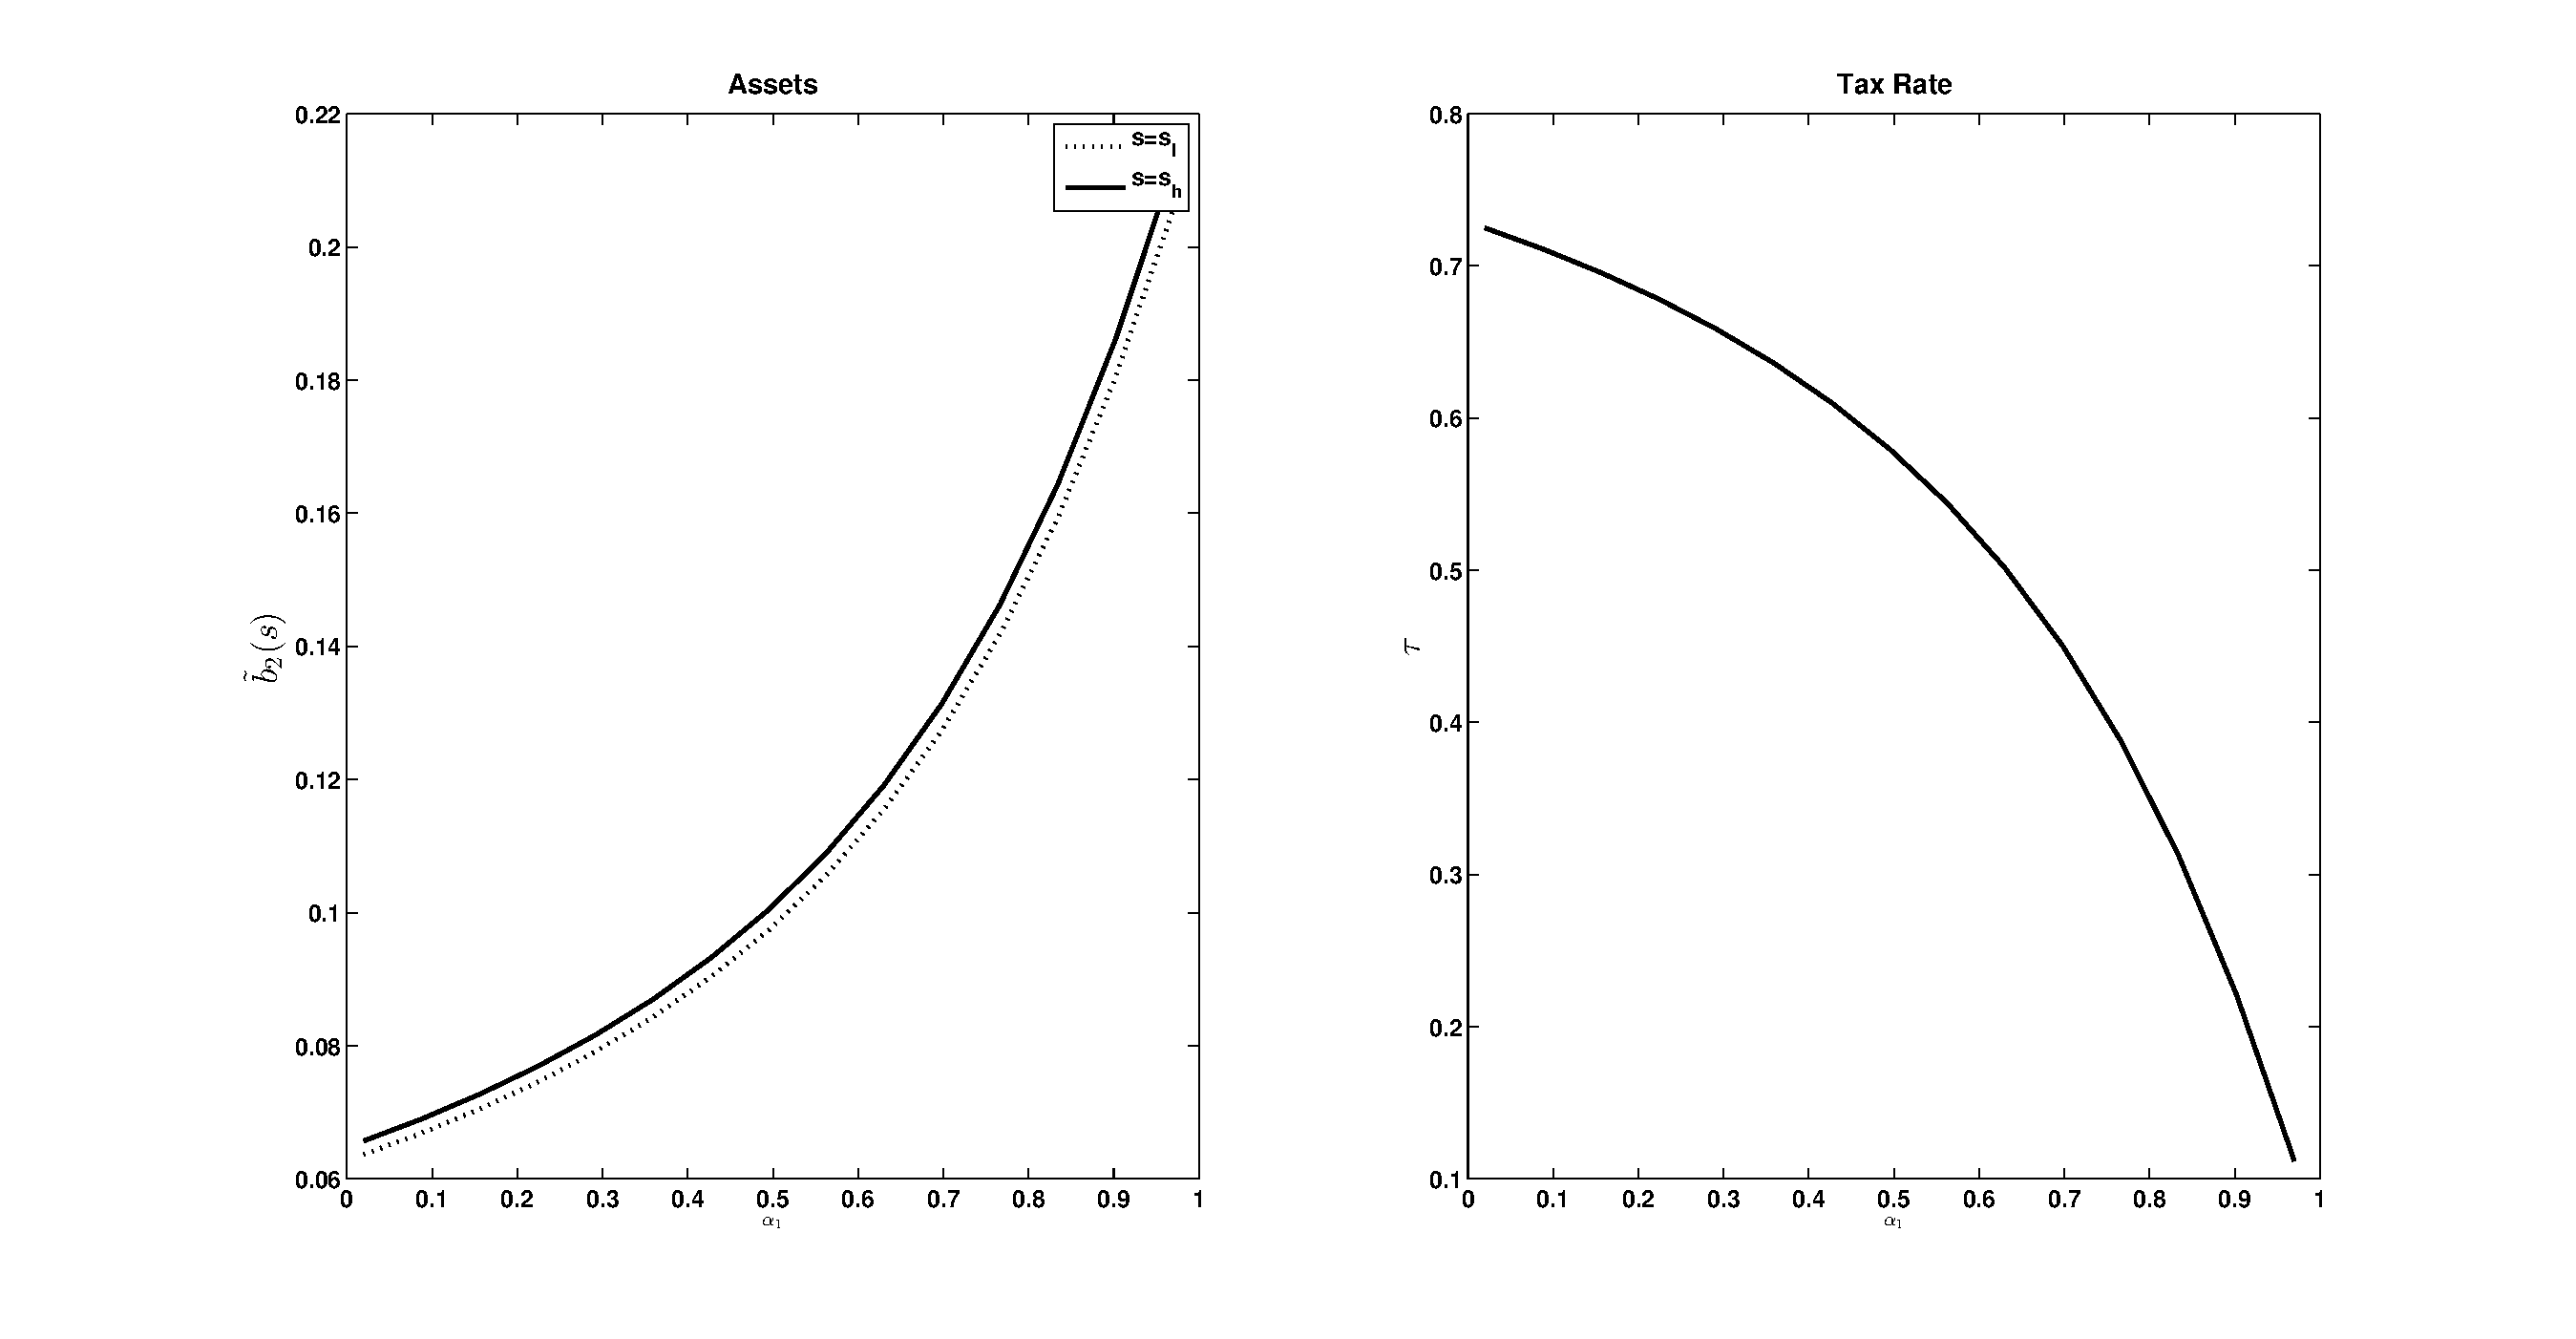
\includegraphics[width=\textwidth]{Draft25Graphs/SS_alpha1.eps}
 \caption{ Stead state assets : $\tilde{b}_2(s)=\frac{\beta  x^{SS}}{U^2_c(s)}$ and taxes : $\tau^{SS}$ as a function of Agent 1's (high skilled) Pareto weight}
 \label{fig: SS comparative}
 \end{figure}

\end{frame}


% \begin{frame}
% \frametitle{ case 1}
% 
% 
% Start with a spread in discount factors such that interest rates are equalized across i.e $R(s_l)=R(s_h)$. One can show that steady state $x>0$
% 
% \begin{itemize}
%  \item The government can adjust two instruments in response  to an adverse  shock (i.e., a fall in $\theta_1$): it can either increase the  tax rate $\tau $ or it can decrease transfers $T.$ Both responses are distortionary
%  \item When agents' asset holdings are identical, a decrease in transfers  disproportionately
% affects a low-skilled agent, so his marginal utility falls by more than does the marginal utility of a high-skilled agent. 
% \item  Consequently, a
% decrease in transfers increases inequality, giving rise to a cost  not present in  representative agent economies.
% \item  The government can reduce the costs of  inequality distortions by choosing tax rate policies that make the net asset positions of  the high-skilled agent
% decrease over time. 
% \item this makes the two agents' after-tax and after-interest income  become closer, allowing decreases in transfers to have smaller effects on inequality in
% marginal utilities. 
%  \end{itemize}
% 
% \end{frame}

\begin{frame}
 \frametitle{Numerical Example}

 Use a  calibrated version of the economy to 
 \begin{itemize}
  \item Revisit the magnitude of these forces and 
  \item Study optimal policy responses at business cycle frequencies when the economy is possibly far away from the steady state
 \end{itemize}
 \end{frame}
 \begin{frame}
 \frametitle{Numerical Example : Calibration}
Take a 2 shock 2 type economy with preferences $U(c,l)=\psi \log(c)+(1-\psi)\log(1-l)$ and allow $\theta_i(s),\beta(s),g(s)$ to depend to shocks.

 \begin{itemize}
 
 \item Pick the baseline parameters to match some low frequency moments

 \item Calibrate the fluctuations to match recent US recessions (i.e., 1991-92, 2001-02 and 2008-10):

 \begin{enumerate}
  \item The left tail of the cross-section distribution of labor income falls by more than right tail
  \item Short term interest rates fall
  \item Recessions last longer than booms
 \end{enumerate}

 \end{itemize}

\end{frame}



\begin{frame}
 \frametitle{Calibration}
 
{\tiny
\begin{table}[htp]
{\tiny
\begin{tabular}{|l|l|l|c|}
\hline
Parameter & Value & Description &Target   \\ \hline
$\psi$ & 0.6994 &Frisch elasticity of labor supply & 0.5   \\
$\bar{\theta}_1 $ & 4& Log 90-10 wage ratio (Autor et all) & 4   \\
$\bar{\theta}_2 $ & 1 &Normalize to 1 & 1  \\
$\beta$ & 0.98  &Average (annual) risk free interest rate & 2\%   \\
$\alpha_1$ & 0.69 & Marginal tax rate in the economy with no shocks & 20\% \\
$g$ & 12\%&Average pre-transfer expenditure- output ratio & 12 \% \\
$\frac{\hat {\theta}_2}{\hat {\theta}_1}$ & 2.5 & Relative drop in wage income of 10th
percentile & 2.5\\
$\hat{\theta}_1$ & 1.2\% & Average output loss& 3\% \\
$\hat{\beta}(s)$ & 1.96\%& Difference in real interest rates between booms and recession& 1.96\% \\
$P(r|r)$ & 0.63&Duration of recessions & 2.33 years \\
$P(b|b)$ & 0.84 &Duration of booms &7 years \\ \hline
\end{tabular}
}
\caption{Benchmark calibration}
\label{tab:Parameters}
\end{table}
}
We initialize the economy with initial conditions such that implied debt to GDP ratio is 60\%
 \end{frame}

\begin{frame}
 \frametitle{Results: Some variants }
 From the Benchmark calibration we will study the following variants
 \begin{enumerate}
\item Acyclical interest rates : Smaller spread in discount factor shocks
\item Countercyclical interest rates: No discount factor shocks 
\item No inequality: Equal fall in all agents productivities (TFP shock) and no discount factor shocks
\item Government expenditure shocks: A fall in $g$ that produces a comparable fall in output 
\end{enumerate}

 \end{frame}

 
\begin{frame}
 \frametitle{Results : Long run}
 
  \begin{figure}[htp]
 \centering
 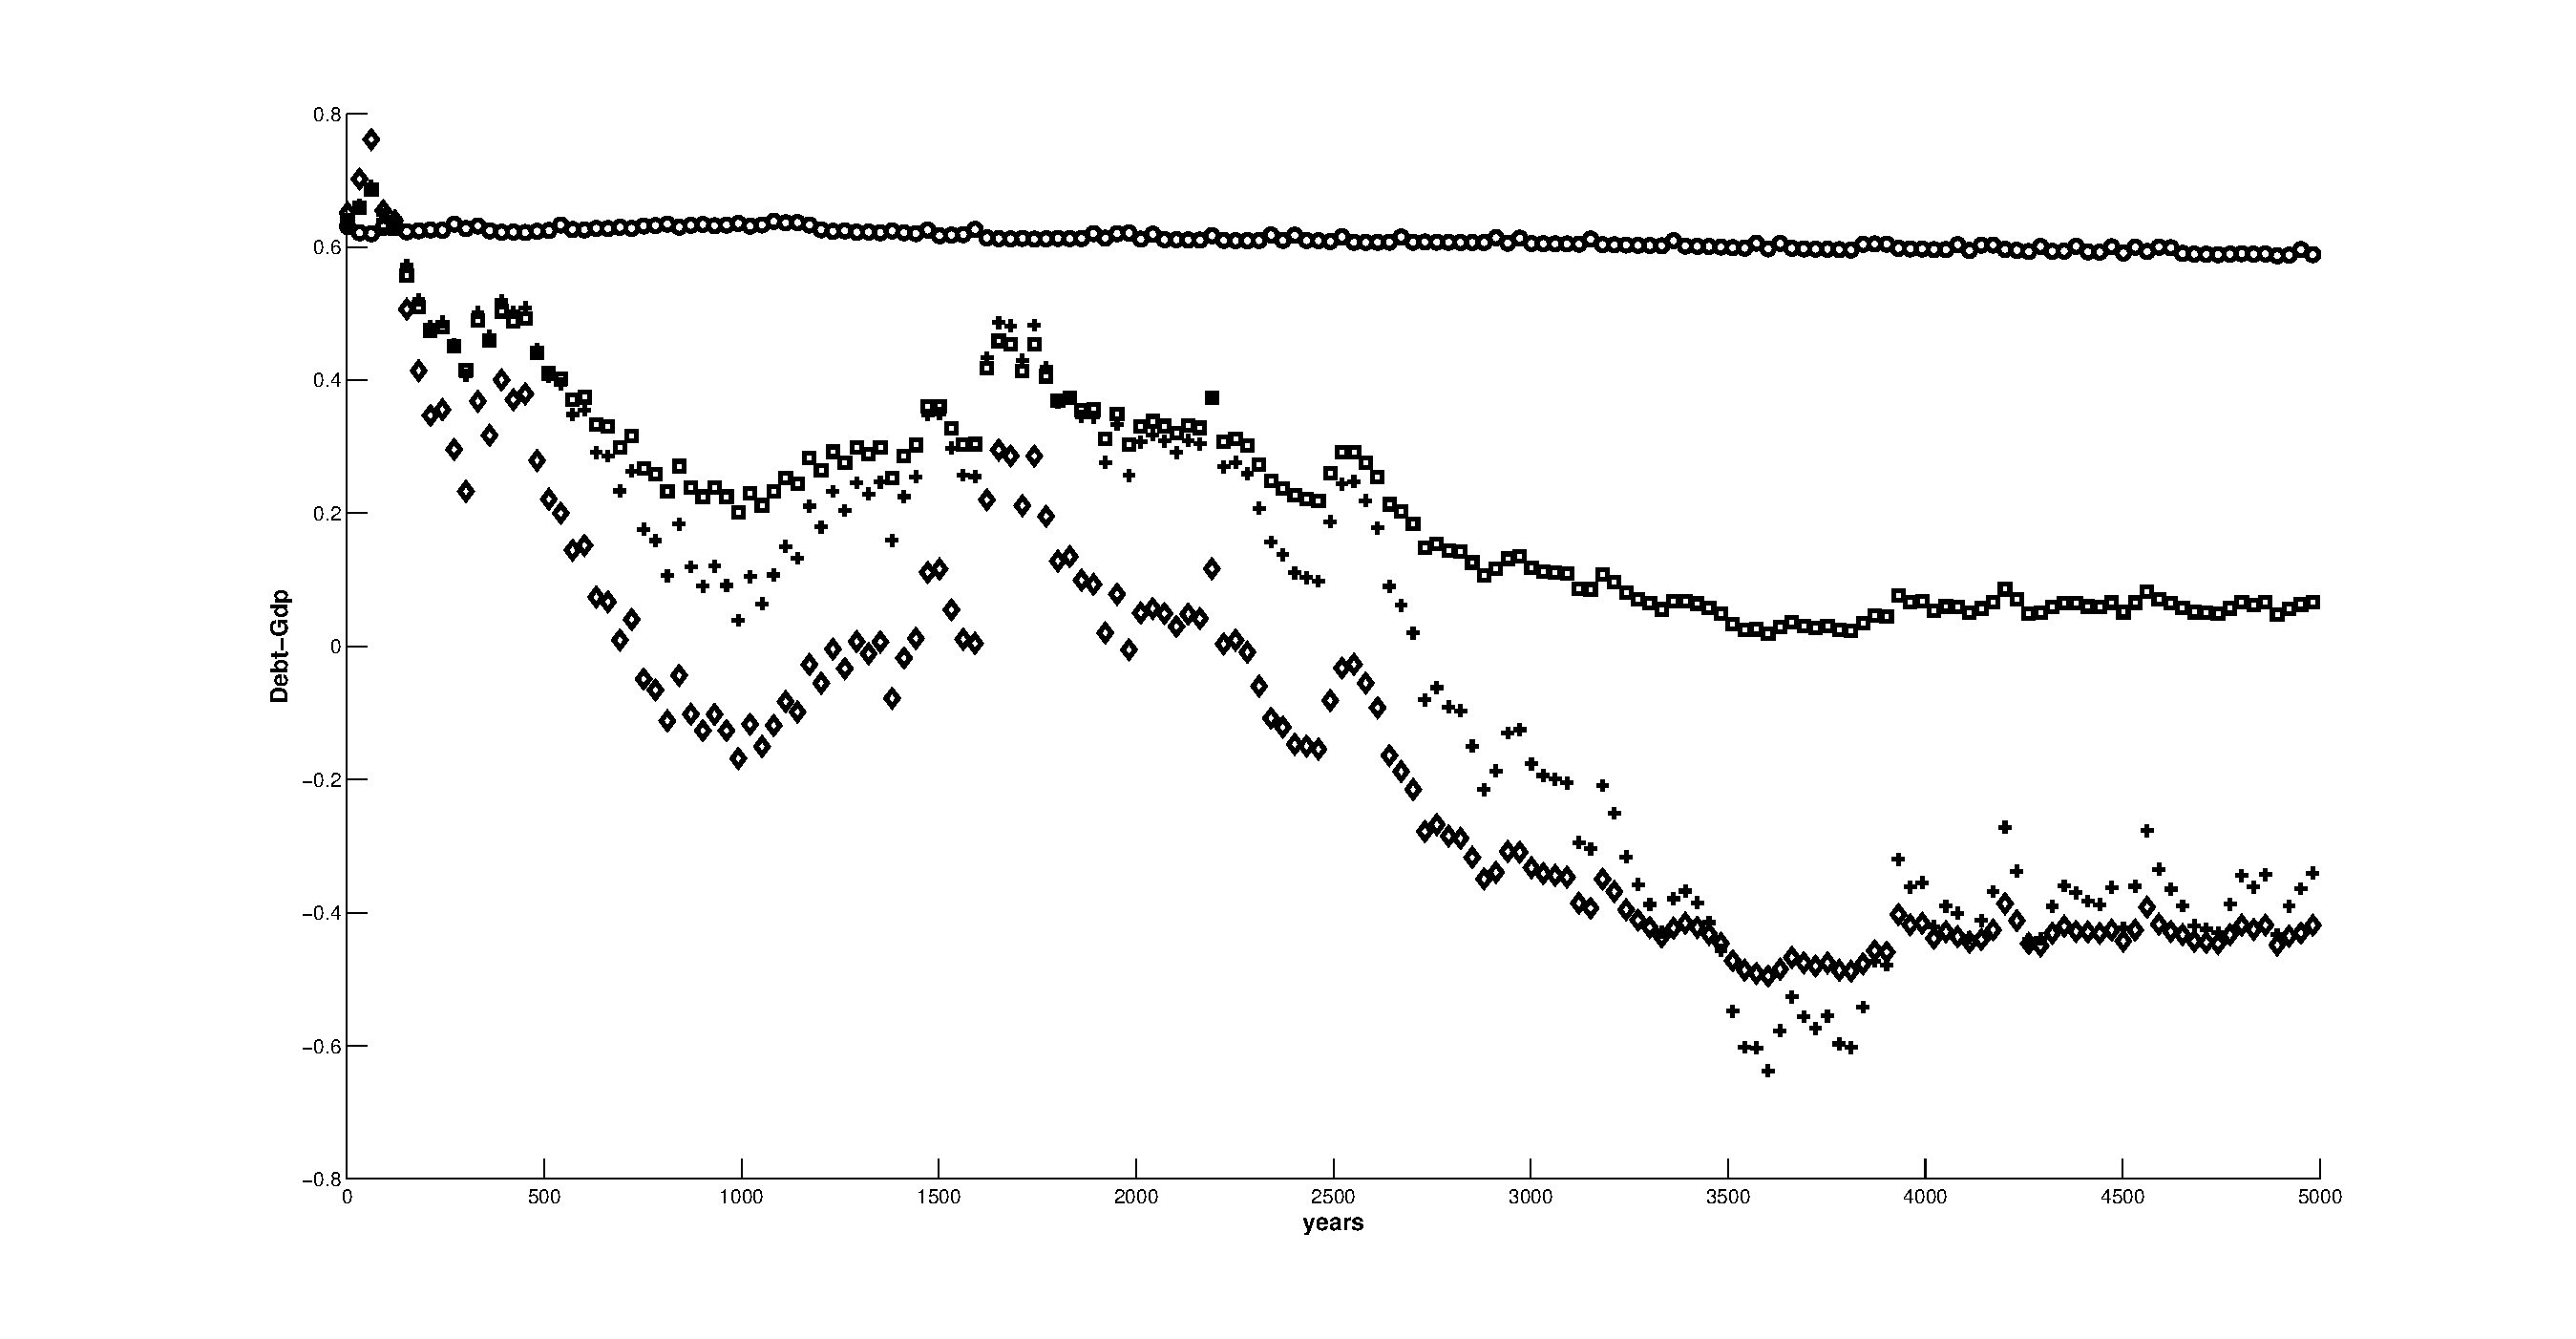
\includegraphics[width=\textwidth]{Draft25Graphs/LongSimulations.eps}
 \caption{Debt benchmark (o), acyclical interest rates (+), countercyclical interest rates ($\diamond$) and no inequality shocks \scriptsize ($\square$\normalsize) }
 %\caption{ Debt benchmark $\circle$, acyclical interest rates + , countercyclical interest rates $\diamond$ }% and no inequality shocks {\scriptsize $\square$ \normalsize}}
 \label{fig:LongSimulations}
 \end{figure}


 \end{frame}
 
 \begin{frame}[label=main]
  \frametitle{Remarks}
  \begin{itemize}
   \item Long run tendency to converge to some ergodic set. But convergence is very slow
   \hyperlink{convergence}{\beamerbutton{more details on speed of convergence}}.
   \item With low discount factor shocks the trend is towards positive assets
   \item With high discount factor shocks that produce procyclical real interest rates there is no tendency to reduce debt even after 5000 years
  \end{itemize}

 \end{frame}

 \begin{frame}
  \frametitle{Short Run}
  To understand the shor run responses, 
  \begin{itemize}
   \item   We set the exogenous state $s_0$ so  that we are at the outset of a recession
   \item Solve the time 0 problem with identical initial conditions across
different settings. This pins down the initial state vector  $x_0,\rho_0$  that appears in our time $0$ Bellman equation
\item We then use the policy rules to compute fluctuations of
different components in the government budget constraint across states
  \end{itemize}
For each variable
$z$ in the table we report in the form $\Delta z\equiv \left( z\left(
s_l|x_0,\rho_0,s_0\right) -z\left( s_h|x_0,\rho_0,s_0\right) \right) /\bar{Y}
$ where $\bar{Y}$ is average undistorted GDP in percentages
 \end{frame}

 
 \begin{frame}
 \frametitle{Results : Short run}
 {\tiny
\begin{table}[tbp]
\begin{tabular}{|l|c|c|c|c|c|c|c|}
\hline
& \textbf{$\Delta g$} & \textbf{$\Delta B$} & \textbf{$\Delta T$} & \textbf{$%
\Delta [\tau\theta_1l_1]$} & \textbf{$\Delta [\tau\theta_2l_2]$} & \textbf{$%
\Delta Y$} & \textbf{$\Delta \tau$} \\ \hline
\textbf{Benchmark} & 0.0000 & -1.1561 & 0.6871 & -0.1593 & -0.3096 & -2.8536
& 0.3732 \\ \hline
\textbf{Acyclical Interest Rates} & 0.0000 & -1.1126 & 0.6591 & -0.1497 &
-0.3038 & -2.8613 & 0.3879 \\ \hline
\textbf{Countercyclical Interest Rates} & 0.0000 & -1.0794 & 0.6387 & -0.1415 &
-0.2992 & -2.8677 & 0.3997 \\ \hline
\textbf{No Inequality} & 0.0000 & -0.1380 &\color{red}{\textbf{ -0.5459}} & -0.5635 & -0.1204 &
-2.6294 & 0.0622 \\ \hline
\textbf{Expenditure Shocks} & -7.5037 & 2.9137 & 2.8612 & -1.3759 & -0.3530 & -2.3443 &
-1.1598 \\ \hline

\end{tabular}%

\caption{The tables summarizes the changes in the different components of the government budget as we transit from ``boom'' to a ``recession''.  All numbers are normalized by un-distorted GDP except $\protect\tau $ and reported in percentages.
}

\label{tab:ShortRunPolicyResponses}
\end{table}
}
Note that predetermined variables like repayment on existing debt drop out
of the accounting and we have
\begin{equation*}
\Delta [g]+\Delta[T]+ \Delta [B]=\Delta[\tau \theta_1 l_1]+ \Delta[\tau
\theta_2 l_2]
\end{equation*}%

 \end{frame}

\begin{frame}
 \frametitle{Conclusions}
\begin{itemize}
\item Size of government debt alone is not informative $\Longrightarrow $
need to know the net distribution of assets in the economy
\item The optimal tax and transfer scheme balances 
\begin{enumerate}
 \item welfare losses from fluctuating taxes
 \item welfare losses from fluctuating transfer
\end{enumerate}
\item Since the welfare costs depend on the how debt is distributed, there are incentives to affect the net assets overtime
\item With incomplete markets, interest fluctuations turn out to be key for the long run correlations between productivities and net assets
\item Ignoring heterogeneity produces misleading results about size and direction of short run optimal policy response
\end{itemize}

\end{frame}
\appendix
\section{More}

\begin{frame}[label=convergence]
\frametitle{Speed of convergence  (I) }
Suppose we are in the binary-IID world where steady states are deterministic. 


\begin{itemize}
\item The optimal policy induces two risk adjusted martingales $\{\bm{\mu}_{t},\bm{\rho}_{t}\}$. 
 \item One can represent the optimal allocation recursively in terms of $\{\bm \mu(s^{t-1}),\bm \rho(s^{t-1})\}$ and $s_t$. 
\item Why $(\bm{\mu},\bm{\rho})$ instead of $(\bm{x},\bm{\rho})$ ?
\item Linearize optimal policies for each $s_t$ around the degenerate steady state. 
\item Study the eigenvalues of the conditional mean and variance dynamics (there are deterministic linear systems)
\end{itemize}

\end{frame}


\begin{frame}
\frametitle{Speed of convergence  (II) }
 $\hat{\Psi}_{t}= \left[\bmat \bm{\mu}_{t} - \bm{\mu}^{SS}\\ \bm \rho_t - \bm \rho^{SS}\emat\right]$ be  deviations from a steady states
\begin{equation*}
 \hat{\Psi}_{t+1}=B(s_{t+1})\hat{\Psi}_t
\end{equation*}
This linearized system has coefficients that are functions of the shock. 
\small
We have 
\begin{proposition}\label{prop: localstability}
If the (real part) of eigenvalues of $\mathbb{E}B(s)$ are less than 1,  the system  converges to zero  in mean. Further for large $t$, the conditional variance of $\hat{\Psi}$, denoted by $\Sigma_{\Psi,t}$, follows a deterministic process governed by
\[\text{vec}(\Sigma_{\Psi,t})=\hat{B} \text{vec}(\Sigma_{\Psi,t-1}),\]	
where $\hat{B}$ is a square matrix of dimension $(2N-2)^2$. In addition,  if the (real part) of eigenvalues of $\hat{B}$ are less than 1, the system converges in probability.
\end{proposition}

\color{red}\emph{The eigenvalues (in particular the largest one) are instructive not only for whether the system is locally stable but also how quickly the steady state is reached}

\end{frame}

\begin{frame}
\frametitle{Speed of convergence : Size of shocks and risk aversion}
  \begin{figure}[htp]
 \centering
 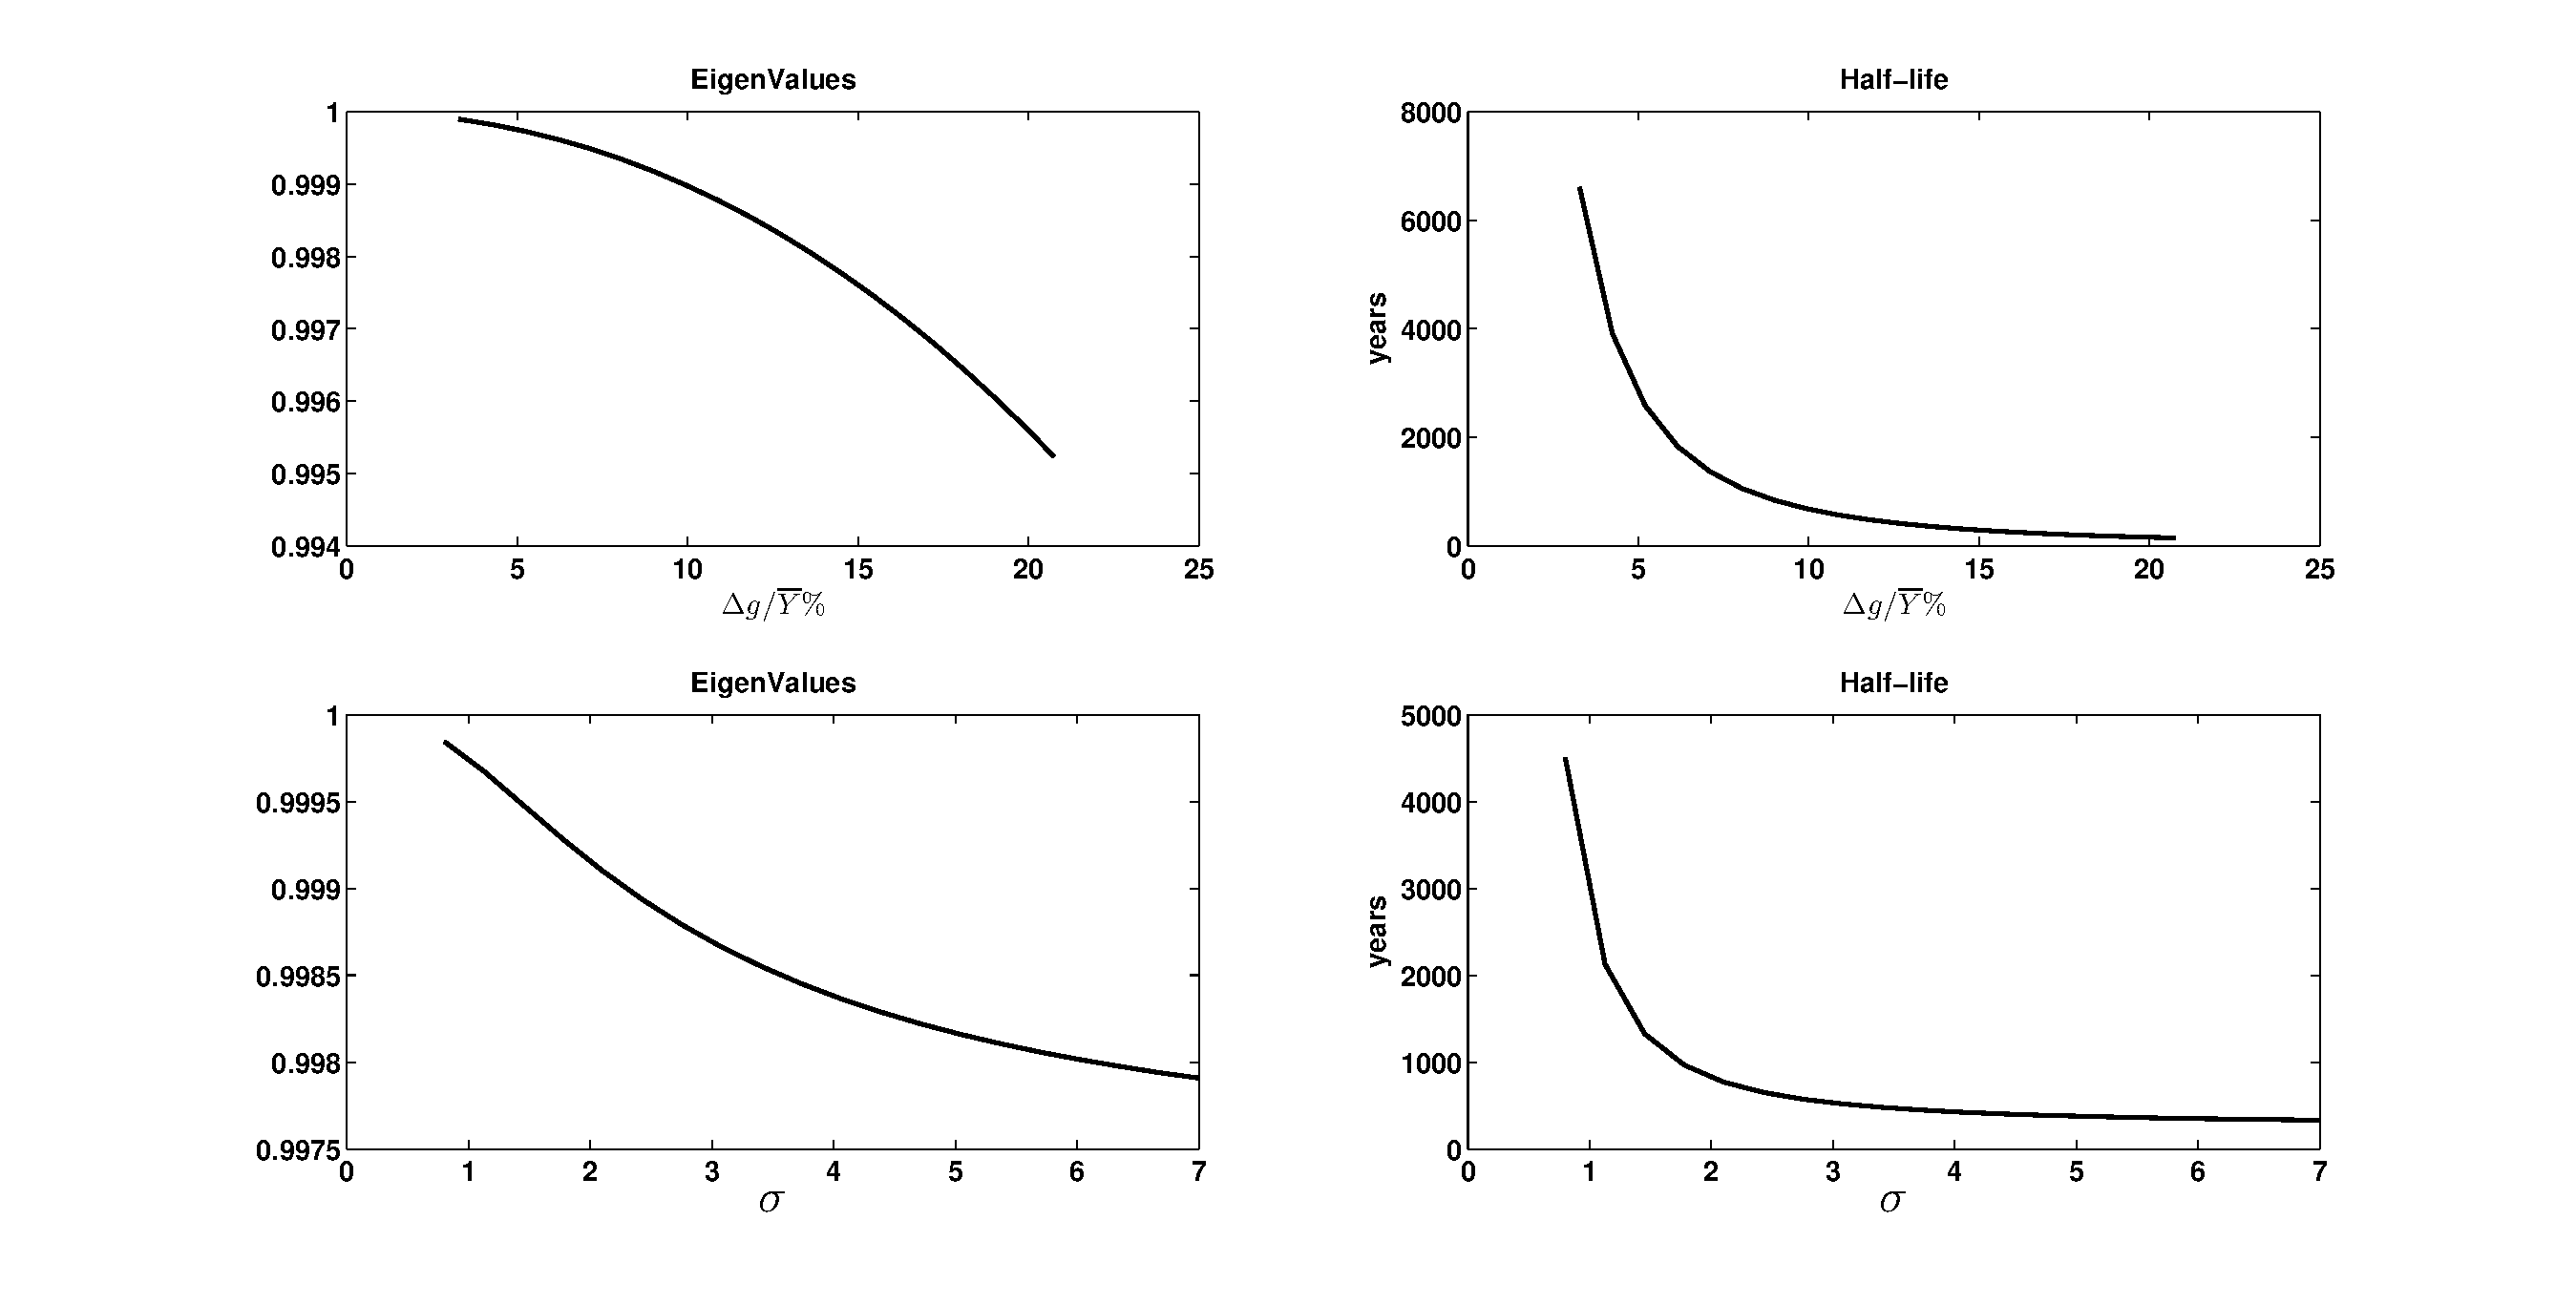
\includegraphics[width=\textwidth]{Draft25Graphs/eigenvalues.eps}
 \caption{The top (bottom) panel plots the dominant eigenvalue of $\hat{B}$ and the associated half life as we increase
the spread between the expenditure levels (risk aversion). }
 \label{fig: Eigenvalues}
 \end{figure}
 Back to \hyperlink{main}{\beamerbutton{main}}.
 \end{frame}
 \end{document}

% 
% \begin{itemize}
% \item Size of government debt alone is not informative $\Longrightarrow $
% need to know the net distribution of assets in the economy
% 
% \item Ignoring heterogeneity produces misleading results about size and
% direction of the optimal policy response
% 
% \item The better ability we have to tax assets, the less debt matters and
% can approximate complete markets closer
% \end{itemize}
% 
% %TCIMACRO{\TeXButton{EndFrame}{\end{frame}}}%
% %BeginExpansion
% \end{frame}%
% %EndExpansion
% 
% \end{document}
